\documentclass[final_report.tex]{subfiles}

\begin{document}

\section{DPDK Java}
\label{sec:implementation}
Since the Data Plane Development Kit is a framework, it was decided that instead of implementing separate middleboxes, a Java framework would be implemented. This would allow any number of other applications to be designed with ease. The DPDK Java framework only supports a subset of the original DPDK features, however, it provides suitable functionality to produce a fully working application which can make use of the key concepts. A number of example applications are implemented in section \ref{sec:apps} using the DPDK Java framework, all of which are easy to extend into more complicated applications which support features like packet fragmentation and packet payload inspection.

\subsection{Overview}
As proven earlier in the report, for fast packet processing in Java the number of JNI calls should be minimised as possible due to their large overhead. However, since DPDK is a native library some JNI calls were obviously mandatory, mainly those initialising the application and packet interactions. This was minimised by making the majority of the JNI calls at the start of the application, before individual processing threads had been started. From then on, JNI calls would only be made at vital times within the application.

An overview of the DPDK Java structure is shown in figure \ref{fig:overview} which shows the key concepts of the framework. Any application requires 2 user defined class:

\paragraph*{Application Main} This class is responsible for starting the DPDK framework indirectly, via a number of method calls to the application starter, passing the required configurations as parameters. Some of this is done via the config file and other properties have to be passed as parameters to the application starter class by the user. It also initialises the custom processor unit class described below and passes them to the application starter. A statistics module can be initialised at the start as well which runs on its own thread.

\paragraph*{Processor Unit} This class is the main unit of the application which is eventually threaded by the framework. It therefore has to extend the Runnable class. It's responsible for requesting packets, processing them and then sending or freeing the packets. These classes can share the Packet Free-er and Packet sender classes but most have their own receive poller class which is associated with a given port and queue.

As figure \ref{fig:overview} shows, most of these classes interface with the native methods, either on a regular basis or on initial start-up. Most of these native methods interact with the DPDK framework in some capacity. However, these native methods are abstracted away from the users application requiring no knowledge of the JNI calls or the underlying memory layout.

\begin{figure}[H]
	\centering
	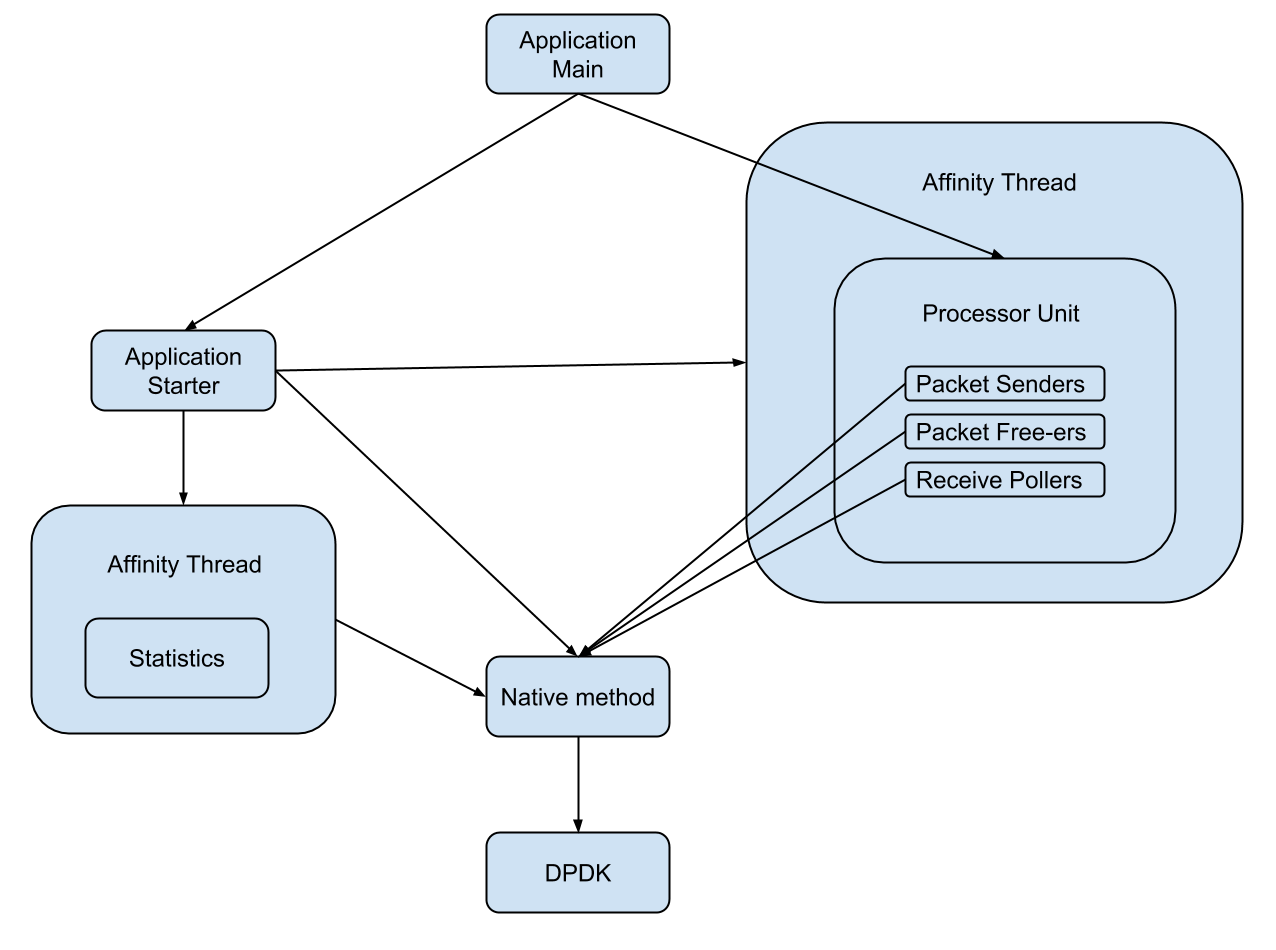
\includegraphics[width=\textwidth]{img/app.png}
	\caption{DPDK Java basic class overview}
	\label{fig:overview}
\end{figure}

\subsection{Native Libraries}
For the Java framework to work, it requires a native shared library which includes all of the native methods to be called. This shared library can be placed anywhere as long as the correct Java path is set to its location, however, the common place is to install it within the users library directory (/usr/lib/) in Linux.

This shared library must also be dynamically linked to other shared libraries which contain the other non-JNI methods called, whether this is system calls, standard system libraries or the actually compiled DPDK libraries. For this, there a number of tools which can be used, all with their own advantages and disadvantages.

\subsubsection{Library Compilation Tools}

\paragraph*{GNU Linker}
The GNU linker on linux is a basic linker which can be used with any number of shared libraries, although as the number increases so does the number of number of commands needed, as well as the number of flags needed. Considering the large amount of shared libraries which DPDK uses, this option is less attractive.

\paragraph*{GNU Libtool}
The GNU Libtool uses the GNU linker underneath but abstracts away the compilations into a build unit, similar the makefiles used. It also has the advantage of only recompiling those libraries required if certain source files are updated. However, it does require a significant amount of set-up, and problems can occur when migrating to other machines.

\paragraph*{DPDK Makefile}
By far the best option is to use the DPDK makefile. It is generally used when the application is written in C and uses the DPDK libraries which is why a lot of documentation is provided on this. However, when wanting to compile shared libraries (which don't include a main method) there is very limited documentation on this and certain flags and processes can only be found by delving into the build process of DPDK. Even so, this is the easiest option to use on a regular basis and ports perfectly well to other systems as it installs the shared library for you as well.

\subsection{Initialisation}
DPDK requires a number of initialising procedures to create the environment abstraction layer, start ports, allocate memory pools and setup the port specific queues. Each of these procedures is directly mapped to a Java implementation of them, which also handle error checking. Generally any native applications using DPDK create a number of threads depending on the number of available cores to split the work and maximise throughput. However, since the Java side creates its own affinity threads for this, DPDK is always initialised with only 1 thread to be used for the set-up.

The native initialisation functions make use of a number of memory allocation (malloc) calls, which goes against the recommended procedures. These calls are used to dynamically create variables such as those used for initialisation parameters for the EAL. After further research into the memory usage, malloc calls are supported and are only discouraged due to the reduced speed of accessing the memory locations over those stored within the huge pages. However, since they are only used at initialisation, performance isn't a factor here.

When writing custom applications, all initialising should be complete before starting the threads. This is to stop any DPDK errors when trying to access uninitialised ports, memory pools or queues. For this reason, the last thing which should be called is 'startAll()' which starts all threads and affinity threads one by one in quick succession to allow the actual packet processing to take place.

\subsection{Processing Threads}
The framework supports multiple processing procedures which can run simultaneously and even with different implementations depending on the requirements. This allows an application to be built where certain processing objects do the polling of packets, and then pass these objects to be inspected, and then onto another object for sending and freeing of the packets. This basically creates a pipelined application, although a more simple processing object would receiver, process and forward packets in the same thread. This is instead of multiple processing units doing exactly the same job.

Each of the processing units are automatically threaded by the framework and put into an 'Affinity Thread'. This follows the same logic of the DPDK framework where each thread is set to only run on 1 core of the machine's processor using affinity cores \todo{ref this and say thread can be set to run on multiple cores - need to fix code for this}. This provided a few complications as Java and the JVM doesn't provide functionality for assignment of threads to cores. This is mainly as because JVM abstracts away the complications of this and allows the kernel to do its own thread scheduling. However, on Linux, Java does utilise the native POSIX Threads (pthread) and assigns a Java thread to 1 pthread. This meant via a few JNI calls and native system calls \todo{example?}, each thread could in fact be associated with certain cores. As with DPDK, this limits the number of threads to be equal or less than the number of available cores on the machine (of hyper-threaded cores) as to fully maximise the application speed.

Each of the processing units must be an extension of the 'PacketProccesor' class which provides an underlying abstraction so statistics of packet data can be retrieved as mentioned below.
\todo[inline]{Describe 3 objects and fix code to use more than 1}

\subsection{Packet Data Handling}
DPDK and therefore the Java framework version is primarily used for packet processing, meaning that efficient handling of the packet's data and header information are a necessity. Investigations outlined in section \todo{ref this} supported that copying packet data from the native side to Java and back again was a very poor choice in terms of processing speed. To solve this, all packet information is left in native memory (not copied to the Java heap) and accessed directly from the Java application in order to read and write data to/from specific packets.

In order to do this, the Java Unsafe class was used extensively as it provided then functionality. However, as discussed previously, the Unsafe class directly accesses native memory and is therefore inherently unsafe to use, as opposed to Java itself. This memory accessing was therefore abstracted away into the 'UnsafeMemory' class which handled the type conversion between native unsigned and Java signed, pointer arithmetic and big/little endian conversion. It also checks whether values are going to be out of data type number representation range when converted from signed to unsigned, since unsigned values are represented as larger data types to account for the signed bit.

Since little-endian to big-endian conversion and vice-versa was required to pass data between the JVM and native memory it was decided that all handling of this would be done on the native side. This firstly abstracts the certain complications of this away from the Java side to provide a cleaner interface and secondly the native implementation provides faster byte shifting. To accomplish this, whenever data was read into a memory location assigned from Java Unsafe, it would flip the data's byte order and put the data into big-endian format for the JVM to interpret correctly. Whenever data was been passed from Java to the native side, the opposite would occur \todo{elaborate on this, diagram? how did pointers work?}.

Each individual network packet is assigned its own Packet object representation. Even though object usage on the Java heap can be relatively slow compared with native structure handling due to various reasons, it was required or else the application would be wondering away from the object orientated side of Java. However, the Packet object only tracks 3 fields in order to minimise data copying:

\begin{itemize}
	\item protected long mbuf\_pointer - points to memory location of the start of mbuf header for the packet
	\item protected long packet\_pointer - points to memory location of the start of the packet header (either IPv4 or IPv6)
	\item protected UnsafeAccess ua - packets own unsafe memory accessing object for secure navigation around packet data
\end{itemize}

Since the native mbuf and ipv4/ipv6 structures are forced to be packed, \todo{ref this} this means that all fields can be traversed and therefore read from and written to via pointer arithmetic. The packet\_pointer allows for simple getters and setters which relate to the standard IP packet headers, even if the actual fields don't exist. The mbuf\_pointer is generally used to gain access to the raw packet data and used later for freeing and forwarding the packet.

\subsection{Packet Polling}
Packet polling as the act of receiving data from the memory buffers used to store packets received by the network interface card/controller. When an application requests new packets from the received queue of a specific port, it does so using native methods via the JNI. These are the only JNI calls used after the initial start up (i.e used in processing threads) in order to increase performance. The native methods' parameters specify the port id, queue id and a memory location pointer, while defaulting to fetching the default number of packets set on the application initialisation. Before this call happens, Java DPDK allocates a set number of bytes within the native memory and holds its pointer in memory in long format. This pointer location is then passed as one of the parameters to the native method.

Within the native method, the number of received packets is put as a short data type into the memory location of the pointer. Every subsequent value inserted into the memory location is first a pointer to the mbuf location of a given packet and then a pointer to the location of the packet header. This happens for all of the packets received by the call.

\begin{figure}[H]
	\centering
	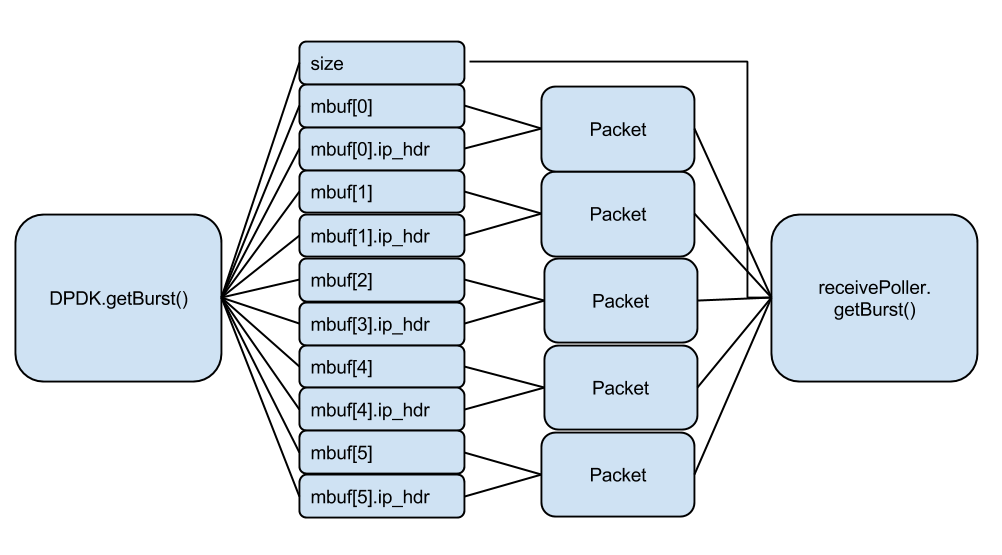
\includegraphics[width=\textwidth]{img/memory.png}
	\caption{Example memory setup for getting burst of packets}
	\label{fig:overview}
\end{figure}

Within the Java side, using the UnsafeMemory class, the number of packets is pulled from the memory location. From there, the pointers can be pulled within a loop and added to their own packet class, depending if they are IPv4 or IPv6 headers. A list of packets is then returned from the method.

\subsection{Packet Sending}
Packet sending involves taking processed packets and putting them on the port queues ready to be sent by the network interface card/controller. When ever a packet needs to be sent, it is passed to a PacketSender object which initiates the process. Within PacketSender, packets are stored within a list ready to be sent. Since packet sending within DPDK is more efficient when sending multiple packets at the same time, whenever the list reaches the default value for a sending burst (n), the first n packets in the list are sent. However, there is also a time-out functionality which is used whenever the receiving of packets is slow. Since the program doesn't want to wait for n packets which could take a long time, the time-out allows any number of packets to be sent if a time reaches a user set time period away from the last send burst.

Sending of packets is very similar to the polling of packets \todo{ref this} but in the opposite direction. Firstly a memory location of the required size (depending on the number of packet to send) is allocated in native memory, and that pointer, along with port id and queue id are passed as parameters to the native code. Each packets' mbuf pointer is then added to the memory location in increasing order. This pointer is then directly passed as a parameter to the DPDK packet sending methods as the memory is already set up in the correct format.

Once the packets have been put onto the queue, a loop if made through the pointers to the mbuf's to free the memory.

\subsection{Statistic Profiling}
The statistic profiling is an optional part of the framework which allows statistics to be gathered on the number and sizes of packets received and packets sent. It gathers data every second by default, but can be user set to find information about the number of packets sent/received for a given time unit. It's up to the user to set which ReceivePoller and PacketSender objects to gather information on. In order to be most efficient for the application, it runs on its own thread, although not an affinity thread, so it can be context switched into any of the cores.

It also has the option of running a graphical user interface (GUI, figure \ref{fig:gui}) which displays the data in better format instead of constant prints to the console. It also redirects other console information on the running of the application to a user console on the GUI for easier use as DPDK outputs a lot of information which isn't that useful.

\begin{figure}[H]
	\centering
	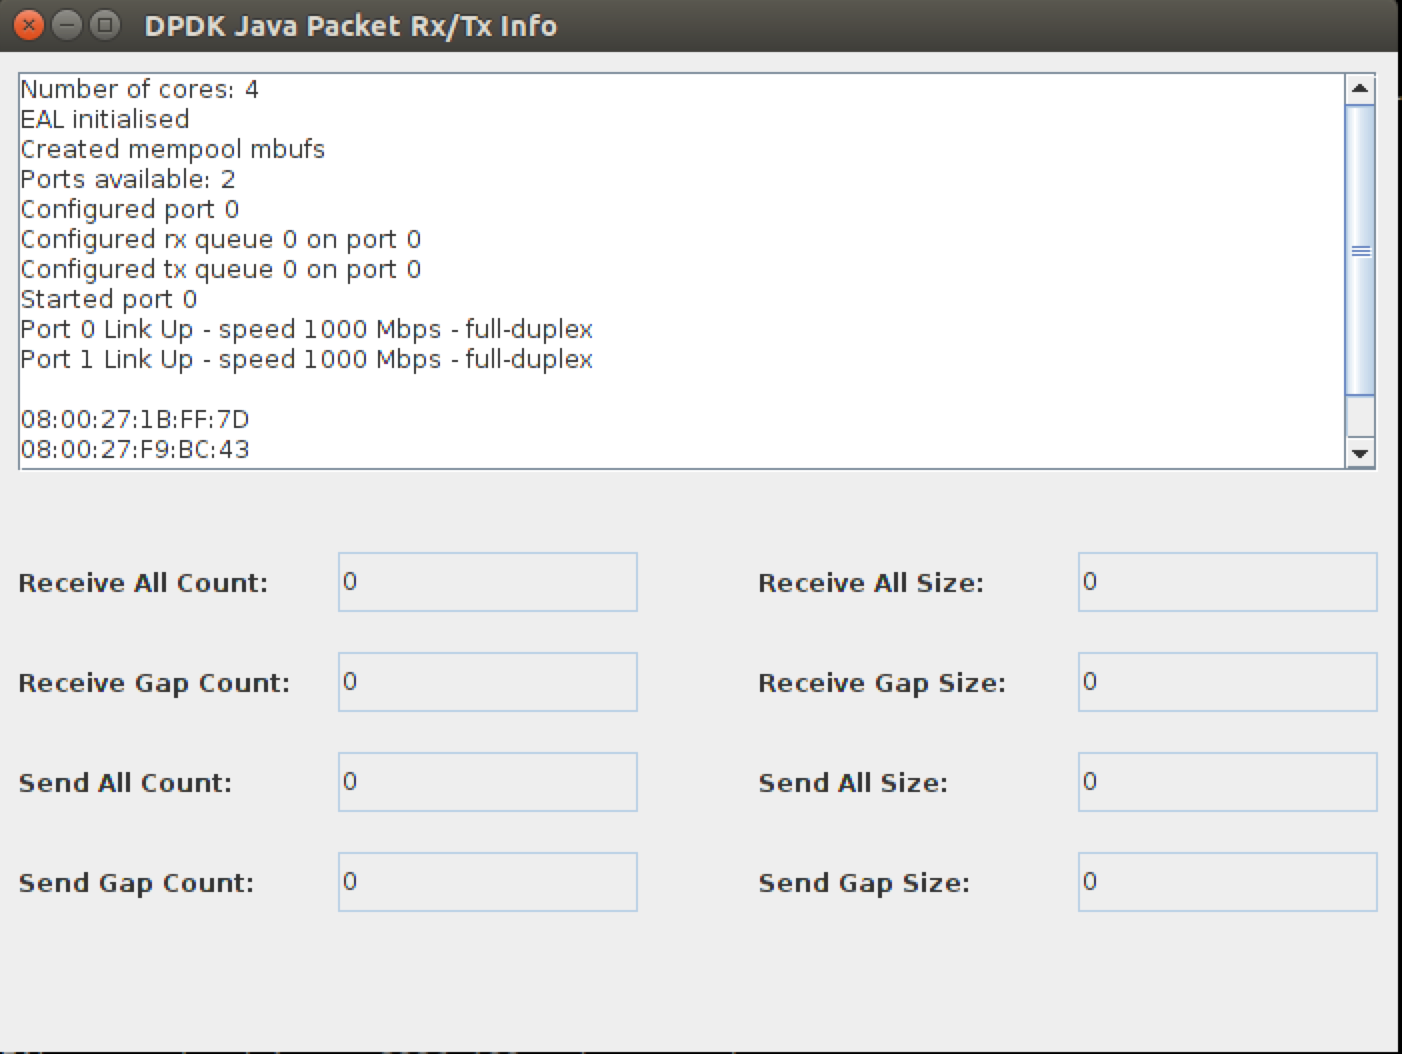
\includegraphics[width=\textwidth]{img/gui.png}
	\caption{Statistics GUI showing packet data and console output}
	\label{fig:gui}
\end{figure}

The implementation for the statistic collector simply involves each packet sender and receive poller iterating counters on the required data. This can potentially have synchronisation issues, which aren't solved to prohibit performance reduction. This means the statistics aren't fully accurate, although they do provide good estimations of the data.

To solve this issue, another statistics profiler was implemented which makes use of some DPDK libraries and native timer libraries to continously poll the NIC for its very accurate on-board data collection. Again, this process is run in a separate thread but it doesn't allow for interaction with the GUI.

\subsection{Correctness Testing}
Not testing performance but packet data movement and pddk set-up
setting u VM since needed specific environments.
%http://www.javacodegeeks.com/2013/02/analysing-a-java-core-dump.html

\subsection{Initial Testing}
The initial testing of applications \todo{which ones?} was carried out an a local Mac OS X machine running Ubuntu 14.04 LTS 64-bit on a VirtualBox \todo{ref this and ubuntu} virtual machine. Although this set-up didn't provide the ability to load test on very high speeds (anything above 1Gbit/s), it allowed for basic testing to check that the application was running as expected. Load testing of speeds up to roughly 700Mbit/s were also possible which have a basic testing platform without the need to move code to servers.

\todo[inline]{important to check for errors at every stage to stop jvm crashes}

\subsubsection{Set-up}
Testing could be carried out using the 2 available 1Gbit NICs of the machine via a bridged network from the host to guest machine which severely reduced transmission speed. This allowed an ethernet cable to be looped back and connected between the ports, meaning anything transmitted via 1 port was guaranteed to be received by the other port.

Pktgen and the custom application were booted up simultaneously running in parallel. Careful memory allocation, port addressing and processor core assignment had to be carried out to stop shared resourced impacting the overall performance of either application. This allowed Pktgen to send packets and the application to receive and process them.

\subsubsection{Methods}

\subsubsection{Results}

\section{Applications}
\label{sec:apps}
Since a Java DPDK framework was designed, any applications are relatively easy to create and only use Java code so no interaction with the native DPDK is necessary from a users point of view. Below are 2 simple applications created using this framework, which both show the small amount of code required to make a working application. However, either of these could be heavily extended to use multiple threads, different processing objects, shared ports in order to design more complex application such as packet fragmentation, reassembly, multi-casting or ordering.

\subsection{Firewall}

\subsection{Network Address Translator (NAT)}

\end{document}
